\documentclass[a4paper,10pt]{article}
\usepackage[utf8]{inputenc}
\usepackage{url}
\usepackage{graphicx}
\usepackage{amsthm}
\usepackage{biblatex}
\usepackage{color}

\bibliography{./rulebib}
%opening
\title{Rule Based Relation Extraction v2}
\author{}

\begin{document}

\maketitle

\section{Backgound}
This writeup discusses an evolved version of the rule based numerical relation extraction system. The basic version of the system is discussed in my mtp report \url{http://www.cse.iitb.ac.in/~amanmadaan/report_aman_mtp1.pdf}, section 11.

\section{Shortcomings of the shortest path hypothesis for numerical relations}
From \cite{shortestpathdep}, \emph{\quotation{If $e_1$ and $e_2$ are two entities mentioned in the same
sentence such that they are observed to be in a relationship R, our hypothesis stipulates that the
contribution of the sentence dependency graph to establishing the relationship $R(e_1, e_2)$ is almost exclusively
concentrated in the shortest path between $e_1$ and $e_2$ in the undirected version of the dependency graph.}}

This hypothesis is bound to break for numerical relations because of the following reasons:

\begin{itemize}
 \item \textbf{The entity $e_1$ can be modified}
 This can be attributed partially to the type of 
 relations targeted, and partially to the type of entities involved. 
 For example, relations with one of the attributes of the type person will almost never involve any modification to the argument.
 
 \item \textbf{Modified relations}
 Numerical relations are highly suspectible to appearing in modified form. It is easier to think of modified forms of 
 relations $height$, $population$ than those of relations like $born\_in$, $employee\_of$.
 \end{itemize}


 Because of these reasons, the shortest path may not be sufficient to capture all the information required to extract a relation.


 For example, consider the sentence, \emph{The diesel price in the Capital of India is 23 \$ per litre}.
 The dependency graph of this sentence is as shown in Fig. 1.
\begin{center}
\begin{figure}[h]
 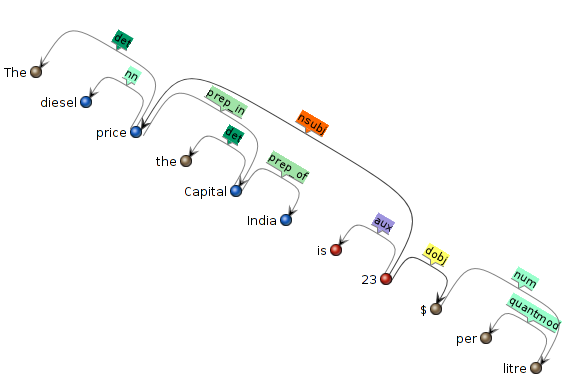
\includegraphics[scale=0.48]{../Pictures/diesel.png}
 % pic.png: 1880x145 pixel, 72dpi, 66.31x5.11 cm, bb=0 0 1880 145
 \caption{\emph{The diesel price in the Capital of India is 23 \$ per litre}}
 \end{figure}
\end{center}
The shortest path between the arguments (India, 23) will be:
\textbf{(Capital, price, 23)}, and thus we'll miss the extraction altogether.

As another example, consider ``Female population of urban india is 23 million''. The dependency graph is as shown in Figure 2.

 \begin{center}
 \begin{figure}
  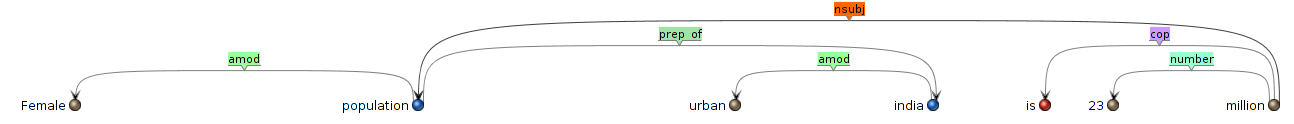
\includegraphics[scale=0.35]{../Pictures/urban_rural.png}
 % urban_rural.png: 1294x124 pixel, 72dpi, 45.64x4.37 cm, bb=0 0 1294 124
 \caption{\emph{Female population of urban india is 23 million}}
 \end{figure}
\end{center}

The shortest path between the arguments  (India, 23) is (Population, million) and thus a vanilla
system will yield the wrong extraction \textbf{\color{red} POP(India, 23 million)}, instead of the correct \textbf{\color{red} POP(urban india, female population, 23 million)}.

As expected, such cases are more of a norm than rarity when dealing with numerical relations, and thus it is imperative that we handle them 
properly.

\section{Obtaining Relation Phrase from keywords and Entity Phrase from country: Modified shortest path hypothesis}

\subsection{Augmented phrases}
Let $S$ be a sentence and $W$ be a word in the sentence. The \emph{Augmented Phrase} $W'$ is formed by concatenating $W$ with words $P$ such that
$W$ and $P$ are related via a \emph{modifying relationship}.

We obtained a list of modifiying relations from the stanford typed dependencies manual \cite{de2008stanford}.
At the moment, the list is restricted to:
\begin{itemize}
\item nn
\item amod
\item vmod
\item advmod
\item dobj
\end{itemize}
We expect the list to grow as we analyze more sentences.

\subsection{The modified shortest path hypothesis}
With definition of augmented phrases as given, we present the modified shortest path hypothesis as follows:
\\
\\
\emph{If $L$ is a location and $N$ is a number mentioned in the same
sentence $S$, \textbf{and} if the shortest path between $L$ and $N$ in the undirected version of the dependency graph of $S$ consists of a keyword 
indicative of a numerical relation $R$, \textbf{and} has no word indicating a change in the numerical quantity, \textbf{and} unit of $N$ is compatible with $R$,
then the sentence expresses the relation \textbf{\color{blue} $R'(L', N)$} where $L'$ is the augmented location phrase and $R'$ is the augmented relation phrase.}

\section{Miscellaneous}

\subsection{Units}
Every relation has a unit associated with it. Before generating an extraction $R'(L', N)$, the unit of $N$ is checked using the unit extractor.

\subsection{Ignoring years}
 At the moment, we treat all numbers from 1950 to 2019 as years and ignore them altogether.
 \begin{verbatim}
(^19[56789]\\d|20[01]\\d)  
 \end{verbatim}

\subsection{Generic Keywords}
Since the keyword phrase is augmented using modifiers, we found it useful to include several generic keywords. For example, 
the keywords for Internet User \% includes ``users, usage and used''. The idea is to first complete the extraction, and then 
perform one final check on the augmented keyphrase extracted. If the keyphrase has ``internet'', call it a valid extraction, otherwise ignore it.

For example, the sentence ``The users in India are 1213.23'' will lead to the extraction \textbf{\color{red} INTERNET(users india, india users, 1213.23)},
but the extractor will ignore it, since the relation phrase doesn't contain ``internet''.

In other words, we supply a set of loose keywords to each relation, in hope that tighter keywords would be connected to them via some modifying relation if the
sentence indeed expresses a relation.


 

\subsection{Aggregating Extractions}
Due to the way the system works, we'll have some work to do before we can populate knowledge bases with the extractions.

\textbf{The urban population of India is 424 million} 

$\rightarrow$ \textbf{\color{red} POP(india, urban population, 424 million)}


\textbf{Urban Indian population stands at 424 million}

$\rightarrow$ \textbf{\color{red} POP(population indian, urban indian population, 424 million)}

We thus need a way to mark the two extractions as the same.


\printbibliography[title=References]


\end{document}
  